\RequirePackage{fixltx2e} %This package in CTeX is not compatible with revtex4-1
\documentclass[aps,pre,12pt,preprint,onecolumn,showpacs,showkeys]{revtex4-1}
\usepackage{ctex}
\usepackage{mathtools}
\usepackage{multirow}
\usepackage{setspace,dcolumn}
\usepackage{hyperref}
\usepackage{graphicx,psfrag,epsfig}
\usepackage[font=small,format=plain,labelfont=bf,textfont=it,justification=centering,singlelinecheck=false]{caption}
\usepackage{amsmath,amsfonts,amssymb,amsthm,bm,upgreek}
\usepackage{geometry}
\usepackage[mathscr]{eucal}
\usepackage{caption}
\usepackage{subcaption}
\hypersetup{colorlinks=true}
\geometry{top=2.54cm,bottom=2.54cm,left=3cm,right=3cm}
\renewcommand\appendixname{附录}
\renewcommand\abstractname{}%摘要
\renewcommand\tablename{表}
\renewcommand\figurename{图}
\makeatletter
\def\@pacs@name{\songti\zihao{-4}{\bf PACS码:}}
\def\@keys@name{\songti\zihao{-4}{\bf 关键词:}}
\def\Dated@name{日期:}
\def\Received@name{\zihao{-5}{接收} }
\def\Revised@name{\zihao{-5}{修订} }
\def\Accepted@name{\zihao{-5}{采纳} }
\def\Published@name{\zihao{-5}{发表} }
\makeatother
\linespread{1.3}
\renewcommand{\labelenumi}{\alph{enumi}.}
\leftmargini=20mm
\def \d {\mathrm d}
\def \degree {^\circ}
\def \V {\bm{V}}
\def \degC {^\circ \mathrm{C}}

\begin{document}
\title{\bf\heiti\zihao{3}非线性热对流斑图\vspace{15mm}}
\author{\fangsong\zihao{4}邵智轩\vspace{2mm}}
\affiliation{\songti\zihao{-4}学号:1400012141\vspace{2mm}}
\date{\today}
%\pacs{02.10.Yn, 33.15.Vb, 98.52.Cf, 78.47.dc}
\keywords{非线性,热对流,线性稳定性分析,瑞利数,阴影法,临界点,斑图}
\email{shaozhixuansh@pku.edu.cn; (86)13381350619}

\begin{abstract}
\vspace{10mm}
\begin{spacing}{1.5}
\songti\zihao{-4}
斑图指的是在时间和空间上具有某种规律性的非均匀宏观结构, 是系统中的微观量相互作用所形成的宏观有序结构. 本实验采用RL-HL20 型氦氖内腔激光器作为光源, CCD 作为记录元件, 通过在2mm 与4mm 薄层水的上下表面维持温差,进行热对流实验, 利用阴影法反映薄层水密度的非均匀分布, 观测到各种对流斑图. 通过改变上下表面的温差, 观察到斑图从无到有的全过程, 同时还观测到了4mm 薄层水中斑图的崩溃过程.
\end{spacing}
\end{abstract}
\maketitle
\songti\zihao{-4}

\section{引言}
	1900 年, 贝纳德 (Benard) 就在具有自由面-固壁底层的流体薄层上进行的热对流实验中观测到了各种对流图形, 后来瑞利 (Rayleigh) 对该系统进行了理论分析, 所以该系统被称为瑞利-贝纳德热对流系统.
	
	瑞利-贝纳德热对流系统中的温度分布不均, 使得流体内部密度分布不均, 产生梯度力, 从而出现热对流. 这是一个非平衡态系统, 由比利时布鲁塞尔学派的代表人物普里高津 (I.Pringogine) 提出的耗散结构理论深化了人们对与这一系统的理解. 耗散结构理论指出: 对于一个远离平衡态的开放系统, 当描述其偏离平衡态的参量越过某一阈值时, 系统会突变到一个稳定有序的状态, 这种结构被称为’ 耗散结构’. 耗散结构理论不仅能解释许多物理, 化学, 生物等自然科学问题, 近年来还被引入到人文社科领域, 成为当代少数几个能横跨自然社会科学的重要科学理论之一. 普里高津也因为这一贡献,获得了1977 年诺贝尔化学奖.
	
	非线性热对流斑图作为耗散结构之一, 在本实验中我们通过阴影法可清晰的观察到. 我们不仅观察2mm 与4mm 薄水层中对流斑图的特点与演化, 还利用线性稳定分析得出转变的临界温度并与实验进行比较, 从而更深入理解耗散结构理论与相关概念.

\section{实验原理}
	\begin{figure}[h]
	\centering
	\includegraphics[width=80mm]{convey.png}
	\caption{\label{fig:convey}%
	上下温度不同的两无限大平板间的热对流系统}
	\end{figure}
	
	图\ref{fig:convey}即为本实验的对流系统示意图。上下两边界为水平,温度分别维持为 $T$ 和 $T+\Delta T$ ($\Delta T > 0$)。
	
	此热对流系统满足鲍兴尼斯克 (Boussinesq) 条件,相应的热对流基本方程组如下:
	\begin{equation}\label{eq:dyn}
		\left\{
		\begin{array}{c}
			\frac{\partial \V}{\partial t}+\V\cdot \nabla\V=g\alpha T \hat{\bm{z}}-\frac{1}{\bar\rho}\nabla p+\gamma \nabla^2 \V\\
			\nabla \cdot \V=0\\
			\frac{\partial T}{\partial t} + \V \cdot \nabla T = \kappa \nabla ^2 T
		\end{array}
		\right.
	\end{equation}
	其中第一个方程有流体力学中的 Navier-Stokes 方程导出,第二个方程为流体连续性方程,第三个方程由热传导方程导出,$\V$为流体速度场,$g$为重力加速度,$\alpha$、$\gamma$、$\kappa$ 分别为液体的热膨胀系数,黏度和热导率,$\bar \rho$ 为流体的平均密度。结合如下的边界条件,
	\begin{equation}\label{bc}
		\left\{
		\begin{array}{c}
			T(z=-d/2)=T+\Delta T \\
			T(z=d/2)=T\\
			V=0,\ z=\pm d/2
		\end{array}
		\right.
	\end{equation}
	动力学方程组\ref{eq:dyn}结合边界条件\ref{bc}有如下定常解:
	\begin{equation}
		T_0 (z)= T_u + \Delta T (1/2- z/d),\quad V_0 =0
	\end{equation}
	而且 $p_0 (z)$ 和 $T_0(z)$ 由以下关系给出:
	\begin{equation} \label{eq:4}
		g \alpha T_0 (z) \hat{\bm{z}} -\frac {1}{\bar \rho} \nabla p_0 (z) =0 
	\end{equation}
	
	我们可以对定态解进行线性稳定性分析。假设存在微扰 $T= T_0 (z) + \theta $,$p= p_0(z)+p'$,$\V=\bm u$代入方程组 \ref{eq:dyn} 并利用 \ref{eq:4} ,去量纲化后得到微扰所满足的方程组:
	\begin{equation}\label{eq:pert}
		\left\{
		\begin{array}{c}
			\sigma^{-1} \left(\frac{\partial \bm u}{\partial t}+\bm u\cdot \nabla\bm u\right)=\theta \hat{\bm{z}}-\nabla p+\nabla^2 \bm u\\
			\nabla \cdot \bm u=0\\
			\frac{\partial \theta}{\partial t} + \bm u \cdot \nabla \theta = \mathrm{Ra} u_z + \nabla ^2 \theta
		\end{array}
		\right.
	\end{equation}
	其中,边界条件为 $\theta=u=0,\ z=\pm\frac{1}{2}$,并定义了瑞利数:
	\begin{equation}\label{eq:Ra}
		\mathrm{Ra}\equiv \frac{g\alpha d ^3 \Delta T}{\kappa \gamma}
	\end{equation}
	
	线性稳定性分析方法将微扰方程 \ref{eq:pert} 中的所有变量视作小量,因此可以忽略非线性项。如此可将方程简化为 $z$ 方向速度分量的方程组,假设初始微扰 $u_z$ 具有如下形式:
	\begin{equation}
		u_z = A(z) \exp [i (k_x x +k_y y ) +st]
	\end{equation}
	其中$|k| \equiv\alpha$,$s$为复数。若解得的$Re(s)<0$,微扰会随时间衰减,原定态解稳定;若$Re(s)>0$,微扰会随时间放大,原定态解不稳定。
	
	方程组 \ref{eq:pert} 是一参量方程,可变参数为瑞利数$\mathrm{Ra}$,它是温度差的函数。当温度差较低时均匀态稳定;当温度高于一临界值时,均匀态不稳定,系统出现斑图结构。通过线性稳定性分析可以求出定态解从稳定到不稳定的临界参数,数值计算的结果为:
	\begin{equation}
		R_c=1707.76,\quad q_c=3.117
	\end{equation}

\section{实验装置}
	\begin{figure}[h]
	\centering
	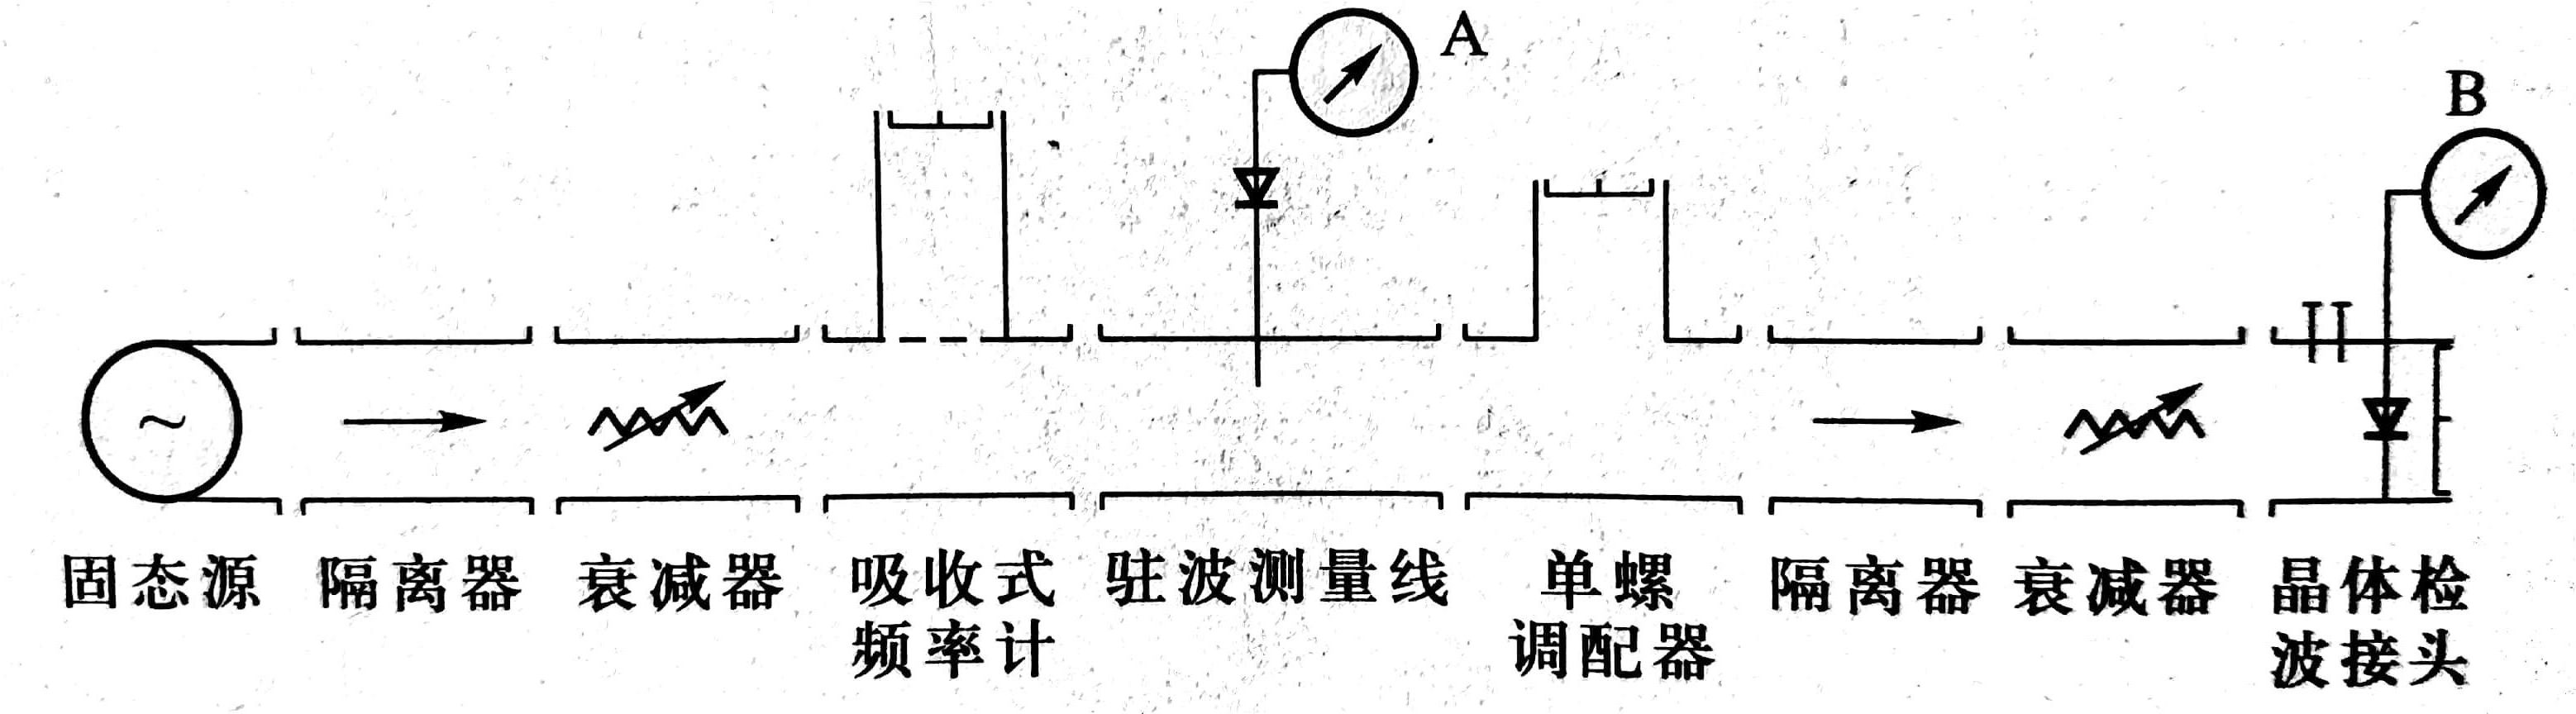
\includegraphics[width=100mm]{equip}
	\caption{\label{fig:equip}%
	非线性热对流斑图实验系统示意图。激光经扩束后被半反半透镜反射照射水层,经水层下表面镀金平面反射后透过半反半透镜在接收屏上成像,通过CCD 收集后观察。}
	\end{figure}
	实验装置如图 \ref{fig:equip} 所示,主要研究对象为夹在降温水层和铜盘之间的对流水层,上层为通过制冷机冷却的降温水层,下部由硅胶加热片加热。为保证水层上下表⾯分别具有均匀的温度,两个水层之间通过蓝宝石片接触,下层使用黄铜盘,都具有较高的热导率。实验中通过设置硅胶加热片的电流控制对流水层上下表面温度差。
	
	本实验采用阴影法来实现液体流场的可视化。当对流水层内出现流动后,其密度出现不均匀分布,从而导致各处的折射率不同,当流场中出现$\frac{\partial ^2 n}{\partial y^2}\ne $常量时,流体对光的作用可看作一个表面曲率非常量的楔形,此时记录平面上的不均匀照明就能反应出流体流动信息。可以直观地理解为折射率较高处,通过相同厚度的水层,光程用更大,该液层位置相当于一块凸透镜,对光线有汇聚作;反之则相当于凹透镜,对光线有发散作用。因此接收屏上亮处对应密度较大的低温区域,暗处对应于密度较小的高温区域。
	
\section{实验内容与结果分析}
	首先调整光路使得接收屏被尽可能均匀照明,同时通过擦拭扩束镜尽量减少干涉条纹带来的影响(然而擦拭后仍然有很明显的衍射条纹)。将 2mm (或 4mm)的黑色 O 环置于黄铜盘上,加入去离子水(预先烧开去除溶解气体),盖上蓝宝石片,需注意观察区域不能有气泡。静候一小时左右以待初始的冲量耗散,使初态尽量接近平衡态。因为制冷剂制冷过程具有暂歇性,难以近似满足实验要求的边界条件,实验过程中并不使用制冷机。由于降温水层温度变化较慢,在较短的时间范围内可以认为满足恒温要求。
	
	本实验分别采用了 2 mm 层和4 mm 水层进行观察。2 mm 和4 mm 水层的加热电流,上下表面温差和斑图描述如表 \ref{tab:2mm} 和表 \ref{tab:4mm}所示;斑图如图 \ref{fig:2mm} 和图 \ref{fig:4mm} 所示。
	\begin{table}[h]
		\caption{\label{tab:2mm}%
		2 mm 水层加热电流, 对流水层上下表面温度差及斑图形状}
		\begin{tabular}{cccccr}
			\hline
			图 \ref{fig:2mm} 中序号&$T_U/\degree \mathrm{C}$&$T_L/\degree \mathrm{C}$&$\Delta T/\degree \mathrm{C}$&$I/\mathrm{A}$&斑图情况\\\hline
			 & 26.4 & 28.3 & 1.9 & 0.250 & 无明显变化 \\
			\ref{fig:2mma} & 28.3 & 34.0 & 5.7 & 0.500 & 无明显变化 \\
			\ref{fig:2mmb} & 28.8 & 35.3 & 6.5 & 0.550 & $\quad$隐隐出现同心圆状斑图,但非常模糊 \\
			\ref{fig:2mmc} & 29.5 & 36.4 & 6.9 & 0.599 & 同心圆变得清晰\\
			\ref{fig:2mmd} & 29.8 & 38.8 & 9.0 & 0.702 & 同心圆变得更清晰\\
			\ref{fig:2mme} & 32.4 & 46.8 & 14.4 & 0.952 & 条纹变得更细锐\\
			\ref{fig:2mmf} & 35.9 & 54.7 & 18.8 & 1.147 & 圆环间距变大,圆向右侧偏 \\\hline
		\end{tabular}
	\end{table}
	
	\begin{figure}[h]
	\centering
		\begin{subfigure}[t]{45mm}
			\centering
			\includegraphics[width=45mm]{mm21}
			\caption{}\label{fig:2mma}
		\end{subfigure}
		\begin{subfigure}[t]{45mm}
			\centering
			\includegraphics[width=45mm]{mm22}
			\caption{}\label{fig:2mmb}
		\end{subfigure}
		\begin{subfigure}[t]{45mm}
			\centering
			\includegraphics[width=45mm]{mm23}
			\caption{}\label{fig:2mmc}
		\end{subfigure}
		\begin{subfigure}[t]{45mm}
			\centering
			\includegraphics[width=45mm]{mm24}
			\caption{}\label{fig:2mmd}
		\end{subfigure}
		\begin{subfigure}[t]{45mm}
			\centering
			\includegraphics[width=45mm]{mm25}
			\caption{}\label{fig:2mme}
		\end{subfigure}
		\begin{subfigure}[t]{45mm}
			\centering
			\includegraphics[width=45mm]{mm26}
			\caption{}\label{fig:2mmf}
		\end{subfigure}
		\caption{2mm 水层斑图的演化.% 在 (a) 中无明显图样;(b) 中已隐隐出现一些同心圆,但由于背景干涉条纹的干扰,不是很清楚;(c) 中同心圆条纹已较清晰;(d) 中条纹更加清晰;(e) 条纹变得细锐;(f) 圆环间距变大
		}\label{fig:2mm}
	\end{figure}
	
	对 2 mm 水层,在温差小于等于5.7 $\degC$时,接受屏一直无明显变化。当温差到达 6.5 $\degC$ 时,在靠近边界处隐隐出现了一些模糊的同心圆条纹,由于背景干涉条纹的干扰,中间的变化看得不是很清楚;进一步加大温差后斑图越来越清晰,细锐,对比度提升,且圆环间距离稍有增大。另一方面,图形的圆对称性有一定程度降低,圆环向右侧偏,这是由于蓝宝石片上的降温水层温度不完全均匀,右侧为入水口,温度较出水口的温度低。
	
	2 mm 水层的温差的临界点在 5.7 $\degC$ 与 6.5 $\degC$ 之间。 没有出现明显的失稳现象。
	
	在测量 4 mm 水层之前,先用冷水机对水箱中的水降温。换上 4 mm O形圈,加去离子水后,仍等待 半小时左右,再开始加热电流。
	
	对 4 mm 水层,在温差小于等于4.9 $\degC$时,接受屏一直无明显变化。当温差到达 7.4$\degC$ 时,出现了一些较模糊的类同心圆条纹;进一步加大温差后斑图越来越清晰细锐,对比度提升,同时出现变形与弯折,暗条纹变成条状,亮条纹呈包状;在温差达到 11.8 $\degC$ 后出现较明显的失稳现象,明暗条纹开始出现交织分叉;当温差加到 20 $\degC$ 附近时,斑图更加混乱,变化更加剧烈,条纹间出现分明的包状小单位的交换。
	
	4 mm 水层的温差的临界点在 4.9 $\degC$ 与 7.4 $\degC$ 之间。 在温差达到 11.8 $\degC$ 左右后出现较明显的失稳现象。
	
	\begin{table}[h]
		\caption{\label{tab:4mm}%
		4 mm 水层加热电流, 对流水层上下表面温度差及斑图形状}
		\begin{tabular}{cccccr}
			\hline
			图 \ref{fig:4mm} 中序号&$T_U/\degree \mathrm{C}$&$T_L/\degree \mathrm{C}$&$\Delta T/\degree \mathrm{C}$&$I/\mathrm{A}$&斑图情况\\\hline
			 & 24.8 & 28.3 & 3.5 & 0.403 & 无明显变化 \\
			\ref{fig:4mma} & 25.2 & 30.1 & 4.9 & 0.502 & 无明显变化 \\
			\ref{fig:4mmb} & 26.8 & 34.2 & 7.4 & 0.600 & 类似于同心圆状的斑图\\
			\ref{fig:4mmc} & 27.9 & 37.2 & 9.3 & 0.699 & 条纹变清晰,同心圆状斑图弯折,变形\\
			\ref{fig:4mmd} & 29.4 & 41.2 & 11.8 & 0.798 & 对比度进一步加大,暗条纹呈条状,亮条纹呈包状\\
			\ref{fig:4mme} & 32.0 & 47.2 & 15.2 & 1.000 & \quad 对比度进一步加大,条纹开始出现分叉,形状不稳定\\
			\ref{fig:4mmf} & 34.3 & 56.0 & 21.7 & 1.194 & 明暗条纹交织分叉,斑图形状极不稳定,快速变化 \\\hline
		\end{tabular}
	\end{table}
	
	\begin{figure}[h]
	\centering
		\begin{subfigure}[t]{45mm}
			\centering
			\includegraphics[width=45mm]{mm41}
			\caption{}\label{fig:4mma}
		\end{subfigure}
		\begin{subfigure}[t]{45mm}
			\centering
			\includegraphics[width=45mm]{mm42}
			\caption{}\label{fig:4mmb}
		\end{subfigure}
		\begin{subfigure}[t]{45mm}
			\centering
			\includegraphics[width=45mm]{mm43}
			\caption{}\label{fig:4mmc}
		\end{subfigure}
		\begin{subfigure}[t]{45mm}
			\centering
			\includegraphics[width=45mm]{mm44}
			\caption{}\label{fig:4mmd}
		\end{subfigure}
		\begin{subfigure}[t]{45mm}
			\centering
			\includegraphics[width=45mm]{mm45}
			\caption{}\label{fig:4mme}
		\end{subfigure}
		\begin{subfigure}[t]{45mm}
			\centering
			\includegraphics[width=45mm]{mm46}
			\caption{}\label{fig:4mmf}
		\end{subfigure}
		\caption{4mm 水层斑图的演化与失稳}\label{fig:4mm}
	\end{figure}
	
	由瑞利数的理论公式 \ref{eq:Ra},当厚度 $d$ 增大为原来的2倍时,相应的临界温差 $\Delta T$ 应为原来的 1/8。我们虽未能测得准确的临界点值,但从范围上来看实验测得的2 mm 与 4 mm 临界值比较接近,绝对不满足理论的比例 1/8 。主要原因可能有:理论推导中假设水层为无限大平面,而实验中有边界的影响;4 mm 水层厚度相对于宽度更大,导致对这一假设的偏离更大。具体来说理论上临界波数 $q_c = 3.117$, 约为 $\pi$, 所以波长约为 $2d$, 在实验中与对流水层尺寸是可比拟的. 同时由于半波长与对流水层厚度成正比, 所以比较上下两排图像, 可发现 d = 4mm 时的明暗条纹间的间距更宽.
	
	另外一个误差来源于,临界点的判定主要依赖于肉眼的分辨,存在着相当大的不确定因素,测 4mm 时,电流步长设置偏大(0.100 $\mathrm A$),范围判断得不够精确;同时扩束透镜难以消去的衍射条纹也影响着临界点附近的成像,从而影响对临界点的判断。
	
	此外,2 mm 未能观察到失稳,而 4 mm 再同样的温差下很明显观察到失稳。这也可以从式 \ref{eq:Ra} 中看出:相同温差下,$\mathrm{Ra}$ 近似增大为原来的8倍,系统处于更远离平衡态的地方。
	
\section{结论}
	通过本实验我们可以清晰的看出斑图的产生直到失稳崩溃的全过程, 观察到了开放系统中的分岔行为,即系统离开原来无序的热力学分支,突变进入一个全新的稳定有序状态;并且对现象做了一些定性的分析,包括随着对流层的厚度的增加, 临界温度会降低, 明暗条纹间距会增大,条纹对比度会增强。加深了对耗散结构理论的认识与非线性理论基本方法的了解. 但由于理论所要求的边界条件实际上并不满足,本实验测得的结果并不与理论值完全契合。

\section{致谢}
	感谢周路群老师对实验的悉心指导,以及在实验过程中的对耗散结构理论、最小熵原理、非线性等问题历史发展和现实联系的生动而富有意义的讲解。同时也感谢我的搭档洛天鹏同学,在实验过程中积极思考、探索与合作。
	
\begin{thebibliography}{}
\bibitem{Book} 吴思诚, 荀坤. 近代物理实验(第四版). 北京:高等教育出版社, 2015
\bibitem{Book} 余志豪, 王彦昌. 流体力学. 北京: 气象出版社, 1982
\end{thebibliography}
\clearpage
\appendix
\section{实验过程思考题}
	\subsection{如何选择硅胶片加热电流?}
		在临界点附近时,减小电流增加的步长(如 0.050 A),这样可以更精确的确定临界点的范围。在远离临界点的参数附近,可适当加大调整步长。
	
	\subsection{如何理解斑图的稳定状态}
		当瑞利数 $Ra$ 大于临界参数 $R_c$ 时,微扰方程中的非线性项不能忽略,需考虑弱非线性作用。用多尺度分析得到扰动振幅所满足的非线性方程,考虑系统的对称性后这种方程的解可以用来理解实验结果的斑图分岔行为。
	
		另外我们也看到,稳定状态下的斑图近似符合系统的圆对称性。
	
\section{实验报告思考题}
	\subsection{随着温差的升高,可看到黑白结构(即斑图)的出现,黑白区域如何对应水层的流动情况?}
		底部温度较高部分的水层上升,对应区域水的密度和折射率较小,而温度较低部分水层下降,对应水的密度和折射率较大。在液体厚度各处保持一致的情形下,光线通过折射率较大部分的光程较大,根据费马成像原理可知该部分将对光线起到汇聚的作用,相当于凸透镜,从而能够看到较亮的白色图案;反之折射率较小的部分则形成黑色图案。综上,白色区域对应于向下流动的冷水,黑色部分对应于向上流动的热水。
	\subsection{斑图出现的临界点如何确定?如何根据所观察的现象确定临界点?}
		临界点为一个零测度量,通过设定某个温度差观察现象的方法理论上无法确定准确的临界点,并且实验成像并非完美,斑图的形成也主要依赖于人眼的判断。本实验中,通过选取一定间隔的温度差的方式确定临界点的大致范围,在可能出现临界点的区域缩小调整参数的步长,从而较为准确地确定临界点。在接收屏上恰好能分辨出有模糊图案形成的温度差即认为是临界温度差。
	\subsection{当水层换成 4 mm 时,考虑临界点会如何改变?并注意实验过程中参数的选择。}
		分析已在正文中给出。
	\subsection{如何确定斑图的空间特征尺度?}
		两暗条纹或两亮条纹间的距离(半波长)便是斑图的空间特征尺度,近似与水层厚度相当。
	\subsection{斑图的空间特征尺度与对流水层厚度的关系如何?}
		根据教材 366 页的条形斑图对应的解的形式:
		\begin{equation}
			\rho(x,y)=\rho_0 \cos qx,\quad \rho(x,y)=\rho_0 \cos qy
		\end{equation}
		注意到理论计算的波数临界值$q_c=3.117$与 $\pi$ 相近,$x$ 是以 $d$ 为单位的无量纲长度,条形斑图的半波长与液层的厚度相当。
\end{document}